\documentclass[12pt,fleqn]{article}
\usepackage{vkCourseML}
\usepackage{gensymb}
\hypersetup{unicode=true}
%\usepackage[a4paper]{geometry}
\usepackage[hyphenbreaks]{breakurl}

\interfootnotelinepenalty=10000

\begin{document}
\title{Лекция 20\\Метрические методы классификации}
\author{Е.\,А.\,Соколов\\ФКН ВШЭ}
\maketitle

\section{Классификатор k ближайших соседей}

Рассмотрим задачу классификации:~$\YY = \{1, \dots, K\}$.
Пусть дана обучающая выборка~$X = (x_i, y_i)_{i = 1}^{\ell}$
и функция расстояния~$\rho: \XX \times \XX \to [0, \infty)$.
Мы не будем требовать, чтобы функция расстояния являлась метрикой~---
достаточно, чтобы она была симметричной и неотрицательной.
Не будем строить модель на этапе обучения, а вместо этого просто запомним
обучающую выборку.
Пусть теперь требуется классифицировать новый объект~$u$.
Расположим объекты обучающей выборки~$X$ в порядке неубывания
расстояний до~$u$:
\[
    \rho(u, x_u^{(1)})
    \leq
    \rho(u, x_u^{(2)})
    \leq
    \dots
    \leq
    \rho(u, x_u^{(\ell)}),
\]
где через~$x_u^{(i)}$ обозначается~$i$-й сосед объекта~$u$.
Алгоритм~\emph{$k$ ближайших соседей}~($k$ nearest neighbours, kNN) относит объект~$u$ к тому классу,
представителей которого окажется больше всего среди~$k$ его ближайших соседей:
\begin{equation}
\label{eq:knn}
    a(u) = \argmax_{y \in \YY} \sum_{i = 1}^{k} [y_u^{(i)} = y].
\end{equation}

\subsection{Метод парзеновского окна}
Проблема формулы~\eqref{eq:knn} состоит в том, что она никак не учитывает расстояния до соседей.
Действительно, если рассматривается~$7$ ближайших соседей, и для объекта~$u$
ближайшие два объекта находятся на расстоянии~$\rho(u, x) \approx 2$,
а остальные~--- на расстоянии~$\rho(u, x) \geq 100$,
то было бы логично обращать внимание только на первые два объекта.
Чтобы добиться этого, можно ввести веса в модель:
\begin{equation}
\label{eq:knnWeighted}
a(u) = \argmax_{y \in \YY} \sum_{i = 1}^{k} w(i, u, x_u^{(i)}) [y_u^{(i)} = y].
\end{equation}
Веса можно делать затухающими по мере роста номера соседа~$i$~(например, $w(i, u, x) = \frac{k + 1 - i}{k}$),
но лучше использовать расстояния при их вычислении.
Это делается в~\emph{методе парзеновского окна}:
\begin{equation}
\label{eq:knnParzen}
    a(u)
    =
    \argmax_{y \in \YY}
        \sum_{i = 1}^{k}
        K \left(
            \frac{\rho(u, x_u^{(i)})}{h}
        \right)
        [y_u^{(i)} = y],
\end{equation}
где~$K$~--- это ядро,~$h$~--- ширина окна.

\section{Ядровая регрессия}

В методе~$k$ ближайших соседей~\eqref{eq:knnParzen} мы, по сути, максимизировали взвешенную долю
правильных ответов среди соседей при предсказании константой~$y$.
Иными словами, мы старались в каждой точке пространства выбрать такое значение модели,
которое было бы оптимально для некоторой окрестности этой точки.

Попробуем воспользоваться этим соображением, чтобы обобщить подход на задачу регрессии.
Будем выбирать в каждой точке такой ответ, который лучшим образом приближает целевую переменную
для~$k$ ближайших соседей:
\begin{equation*}
    a(u)
    =
    \argmin_{c \in \RR}
        \sum_{i = 1}^{k}
        K \left(
            \frac{\rho(u, x_u^{(i)})}{h}
        \right)
        (c - y_u^{(i)})^2.
\end{equation*}
Можно в явном виде выписать решение оптимизационной задачи:
\begin{equation}
\label{eq:kernelRegr}
    a(u)
    =
    \frac{
        \sum_{i = 1}^{k}
        K \left(
            \frac{\rho(u, x_u^{(i)})}{h}
        \right)
        y_u^{(i)}
    }{
        \sum_{i = 1}^{k}
        K \left(
            \frac{\rho(u, x_u^{(i)})}{h}
        \right)
    }
\end{equation}
Данную модель иногда называют формулой Надарая-Ватсона.

\section{Оптимальность метода kNN}

Рассмотрим задачу бинарной классификации в вероятностной постановке~---
будем считать, что в каждой точке пространства определена вероятность
положительного класса~$p(y = +1 \cond x)$.
Допустим, мы хотим сделать предсказание для объекта~$u$.
Будем считать, что размер обучающей выборки стремится к бесконечности~---
в этом случае для ближайшего к~$u$ объекта~$x_u$ из выборки
распределение~$p(y = +1 \cond x_u)$ слабо отличается от~$p(y = +1 \cond u)$~(мы предполагаем,
что функция распределения непрерывна по~$u$).
Для простоты предположим, что эти распределения совпадают:~$p(y = +1 \cond x_u) = p(y = +1 \cond u)$.
Вероятность ошибки метода одного ближайшего соседа равна
\begin{align*}
    p_\text{1nn}
    &=
    p(y = +1 \cond x_u) (1 - p(y = +1 \cond u))
    +
    (1 - p(y = +1 \cond x_u)) p(y = +1 \cond u)
    =\\
    &=
    2 p(y = +1 \cond u) (1 - p(y = +1 \cond u)).
\end{align*}
Оптимальный байесовский классификатор будет выдавать в точке~$u$ прогноз
\[
    k_* = \argmax_{k \in \YY} p(y = k \cond u).
\]
Вероятность ошибки оптимального классификатора равна
\[
    p_\text{bayes}
    =
    1 - p(y = k_* \cond u).
\]
Отсюда можно вывести, что
\[
    p_\text{1nn}
    =
    2 p(y = k_* \cond u) (1 - p(y = k_* \cond u))
    \leq
    2 (1 - p(y = k_* \cond u))
    =
    2 p_\text{bayes}.
\]
Мы показали, что асимптотически вероятность ошибки метода одного ближайшего соседа в худшем случае в два раза больше,
чем вероятность ошибки оптимального классификатора.
Это утверждение можно показать строго; более того, оно верно не только для бинарной классификации.
Например, для многоклассовой классификации выполнено
\[
    p_\text{1nn}
    \leq
    2 p_\text{bayes}
    -
    \frac{K}{K - 1}
    p_\text{bayes}^2.
\]

Из данных рассуждений следует, что если бы в любой задаче нам было доступно неограниченное количество данных,
то было бы достаточно применить метод одного ближайшего соседа~--- он близок по качеству к оптимальному,
и нет необходимости в других моделях.

\section{Расстояния между текстами}

Основной параметр, от которого зависит качество метрических методов~--- это функция расстояния~$\rho(x, z)$.
Если она выбрана правильно, то kNN может заменить любую другую модель.
Для примера рассмотрим способы измерения расстояний для текстовых данных.

Тексты можно закодировать с помощью мешка слов.
В этом случае каждый текст представляется
в виде вектора длины~$d$~(размер словаря), и~$i$-й элемент этого вектора равен~$x_i = \frac{c_i}{\sum_{k = 1}^{d} c_k}$,
где~$c_i$~--- доля вхождений~$i$-го слова в документ.
После этого расстояние между текстами можно измерять, например, через косинус между их векторами:
\[
    \rho(x, z)
    =
    \frac{
        \langle x, z \rangle
    }{
        \|x\| \|z\|
    }.
\]

Такой подход никак не учитывает, что различные слова могут быть близки друг к другу по смыслу.
Например, фразы~<<Obama speaks to the media in Illinois>> и~<<The President greets the press in Chicago>>
после удаления артиклей и предлогов не будут иметь общих слов, но при этом несут один и тот же смысл.
Фраза~<<The band gave a concert in Japan>> тоже не содержит общих слов, но теперь
её слова по смыслу отличаются от слов из первых двух фраз.

Одна из мер сходства смыслов слов~--- это расстояние между их представлениями~(например, word2vec).
Обозначим такое расстояние между~$i$-м и~$j$-м словами словаря через~$c(i, j)$.

Теперь мы можем определить расстояние между текстами.
Будем считать, что из~$i$-го слова в тексте~$x$ в~$j$-е слово текста~$z$ <<перетекает>> некоторое количество~$t_{ij}$ смысла.
Чем меньше похожи эти слова, тем сложнее перемещать смысл между ними~--- а именно, сложность такого перемещения
зададим как~$c(i, j) t_{ij}$.
Расстояние будет равно минимальной сложности перемещения всех слов первого текста в слова второго:
\[
    \left\{
    \begin{aligned}
        &\rho(x, z) = \min_{t_{ij}} \sum_{i, j = 1}^{d} t_{ij} c(i, j) \\
        &\sum_{j = 1}^{d} t_{ij} = x_i; \\
        &\sum_{i = 1}^{d} t_{ij} = z_j; \\
        &t_{ij} \geq 0.
    \end{aligned}
    \right.
\]
Данную задачу можно решать, например, алгоритмами поиска максимального потока минимальной стоимости.

\section{Методы поиска ближайших соседей}
\subsection{Точные методы}
Разберем методы поиска ближайших соседей для евклидовой метрики.
Будем рассматривать задачу поиска одного ближайшего соседа,
все методы несложно обобщаются на случай с~$k > 1$.

Если просто перебирать все объекты обучающей выборки,
выбирая наиболее близкий к новому объекту, то получаем сложность $O(\ell d)$.

Можно выбрать подмножество признаков, и сначала вычислить расстояние только по этим координатам.
Оно является нижней оценкой на полноценное расстояние,
и если оно уже больше, чем текущий наилучший результат, то данный объект можно больше
не рассматривать в качестве кандидата в ближайшего соседа.
Такой подход является чисто эвристическим и не гарантирует
сублинейной сложности по размеру обучения.

\paragraph{kd-деревья.}
Одной из структур данных, позволяющих эффективно искать ближайших соседей
к заданной точке, является~\emph{kd-дерево}.
Оно разбивает пространство на области~(каждая вершина производит разбиение
по определенной координате), и каждый лист соответствует одному объекту из обучающей выборки.
Обходя это дерево определенным образом, можно найти точку из обучения, ближайшую к заданной.
Если размерность пространства небольшая~($10$-$20$),
то данный подход позволяет находить ближайшего соседа за время порядка~$O(\log \ell)$.

Экспериментально было установлено, что в пространствах большой размерности сложность
поиска ближайшего соседа в kd-дереве сильно ухудшается и приобретает линейный
порядок сложности~\cite{weber98similarity}.

\subsection{Приближенные методы}
Есть два способа борьбы с высокой сложностью поиска ближайших соседей при большом числе признаков:
\begin{enumerate}
    \item Запоминать не всю обучающую выборку, а лишь ее представительное подмножество.
        Существует большое число эвристических алгоритмов для отбора эталонных объектов~(например, STOLP).
    \item Искать~$k$ ближайших соседей приближенно, то есть есть разрешать
        результату поиска быть чуть дальше от нового объекта, чем~$k$ его истинных соседей.
        Ниже мы подробно разберем этот подход.
\end{enumerate}

Опишем метод приближенного поиска ближайших соседей LSH~(locality-sensitive hashing).
Его идея заключается в построении такой хэш-функции для объектов выборки,
которая с большой вероятностью присваивает одинаковые значения близким объектам
и разные значения отдаленным объектам.
Дадим формальное определение.
\begin{vkDef}
    Семейство функций~$\FF$ называется~$(d_1, d_2, p_1, p_2)$-чувствительным,
    если для всех~$x, y \in \XX$ выполнено:
    \begin{itemize}
        \item Если~$\rho(x, y) \leq d_1$, то~$\PP_{f \in \FF} \left[ f(x) = f(y) \right] \geq p_1$.
        \item Если~$\rho(x, y) \geq d_2$, то~$\PP_{f \in \FF} \left[ f(x) = f(y) \right] \leq p_2$.
    \end{itemize}
    Здесь под вероятностью~$\PP_{f \in \FF}$ понимается равномерное распределение
    на всех функциях семейства~$\FF$.
\end{vkDef}
Отметим, что определение имеет смысл лишь если~$d_1 \leq d_2$ и~$p_1 \geq p_2$.

\paragraph{Пример.}
Рассмотрим пример семейства хэш-функций для меры Джаккарда,
которое носит название MinHash.
Пусть объекты представляют собой множества, являющиеся подмножествами
универсального упорядоченного множества~$U = \{u_1, \dots, u_n\}$.
Выберем перестановку~$\pi$ на элементах этого множества,
и определим хэш-функцию~$f_\pi(A)$ так, чтобы она возвращала
номер первого элемента в данной перестановке, входящего в~$A$:
\[
    f_\pi(A) = \min \{\pi(i) \cond u_i \in A \}.
\]
Это преобразование можно интерпретировать следующим образом.
Будем считать, что элементы наших множеств~--- это слова.
Перестановка~$\pi$ задает~\emph{степени важности} слов~(чем меньше~$\pi(i)$,
тем важнее~$i$-е слово).
Например, если мы решаем задачу классификации текстов на научные
и ненаучные, то предлоги и союзы должны иметь малый уровень важности,
а слова~<<аннотация>>, <<бустинг>>, <<переобучение>>~--- высокий уровень важности,
поскольку их наличие свидетельствует о научности текста.
Описанная хэш-функция возвращает для документа уровень важности
самого важного слова в нем~--- в нашем примере это означает,
что мы находим самое~<<научное>> слово в тексте,
и характеризуем документ именно этим словом.

Покажем, что множество всех MinHash-функций~$\FF = \{f_\pi \cond \pi \in \text{Sym}(U)\}$
является~$(d_1, d_2, p_1, p_2)$-чувствительным.

Сначала докажем следующее утверждение: вероятность того, что случайно
выбранная функция~$f_\pi \in \FF$ будет принимать одинаковые значения
на двух заданных множествах~$A$ и~$B$, равна коэффициенту
Джаккарда~$\frac{|A \cap B|}{|A \cup B|} = 1 - \rho_J(A, B)$ этих
двух множеств.
Разобьем элементы~$u$ универсального множества~$U$ на три типа:
\begin{enumerate}
    \item $u \in A$, $u \in B$.
    \item $u \in A$, $u \notin B$ или $u \notin A$, $u \in B$.
    \item $u \notin A$, $u \notin B$.
\end{enumerate}
Обозначим число объектов первого типа через~$p$, а число объектов второго типа~--- через~$q$.
Заметим, что через~$p$ и~$q$ можно выразить коэффициент Джаккарда для
множеств~$A$ и~$B$: $1 - \rho_J(A, B) = \frac{p}{p + q}$.

Вероятность того, что значения случайно выбранной хэш-функции будут одинаковыми
на множествах~$A$ и~$B$, равна вероятности того, что в случайно выбранной перестановке
множества~$U$ элемент первого типа встретится раньше элемента второго типа;
элементы третьего типа на значение хэш-функции никак не влияют.
Последняя же вероятность равна~$\frac{p}{p + q}$.
Утверждение доказано.

Пусть расстояние Джаккарда между двумя множествами~$\rho_J(A, B)$
не превосходит~$d_1$.
Тогда для коэффициента Джаккарда выполнено~$1 - \rho_J(A, B) \geq 1 - d_1$,
а значит, для вероятности~$p_1$ того, что случайно выбранная функция из~$\FF$ даст
одинаковые хэши для этих множеств, выполнено~$p_1 \geq 1 - d_1$.
Отсюда получаем, что~$\FF$ является~$(d_1, d_2, 1 - d_1, 1 - d_2)$-чувствительным семейством.


\paragraph{Композиция хэш-функций.}
Семейство хэш-функций уже можно использовать для поиска ближайших соседей.
Выберем случайную хэш-функцию~$f$, создадим таблицу~$T$,
и разместим каждый объект обучающей выборки~$x$ в ячейке~$f(x)$
этой хэш-таблицы~\footnote{
    Поскольку множество значений хэш-функции может быть большим,
    обычно таблица~$T$ сама является хэш-таблицей.}.
Пусть теперь требуется найти~$k$ ближайших соседей для объекта~$u$.
Вычислим для него хэш~$f(u)$, возьмем все объекты из соответствующей ячейки хэш-таблицы,
и вернем из них~$k$ ближайших к~$u$.
Однако, как правило, разница между вероятностями~$p_1$ и~$p_2$
оказывается не очень большой, поэтому либо истинные~$k$ ближайших соседей
не окажутся в ячейке~$f(u)$, и результат будет далек от оптимального,
либо в эту ячейку попадет слишком много лишних объектов,
и тогда поиск окажется слишком трудозатратным.

Чтобы увеличить разницу между вероятностями~$p_1$ и~$p_2$,
можно объединять несколько простых хэш-функций из семейства
в одну сложную.
Выберем для этого~$m$ функций~$f_1, \dots, f_m$ из~$\FF$
и построим новую функцию~$g_1(x) = (f_1(x), \dots, f_m(x))$.
Повторим процедуру~$L$ раз и получим~$L$ таких функций~$g_1(x), \dots, g_L(x)$.
Для каждой функции~$g_i(x)$ создадим свою хэш-таблицу~$T_i$,
и поместим каждый объект обучающей выборки~$x$ в ячейку~$g_i(x)$ этой таблицы.
Чтобы найти~$k$ ближайших соседей для нового объекта~$u$,
выберем объекты из ячеек~$g_1(x), \dots, g_L(x)$ таблиц~$T_1, \dots, T_L$
соответственно, и вернем~$k$ наиболее близких из них.

Данный алгоритм имеет два параметра: число базовых функций в одной композиции~$m$,
и число таких композиций~$L$.
Увеличение параметра~$m$ приводит к уменьшению вероятности того,
что два непохожих объекта будут признаны схожими.
Действительно, для того, чтобы значения композиции совпали на двух объектах,
необходимо, чтобы совпали значения~$m$ базовых хэш-функций.
Если расстояние между этими объектами велико, т.е.~$\rho(x, y) \geq d_2$,
то вероятность совпадения значений~$m$ базовых функций не будет превышать~$p_2^m$.
В то же время чрезмерное увеличение параметра~$m$ может привести к тому,
что практически все объекты попадут в разные ячейки хэш-таблицы,
и для новых объектов не будет находится ни одного соседа.

Увеличение же параметра~$L$ приводит к увеличению вероятности того,
что два схожих объекта будут действительно признаны схожими.
Действительно, объект~$x$ будет рассмотрен нашим алгоритмом
как кандидат в~$k$ ближайших соседей для~$u$, если хотя бы
один из хэшей~$g_1(x), \dots, g_L(x)$ совпадет с хэшем~$g_1(u), \dots, g_L(u)$
соответственно.
Если объекты~$x$ и~$u$ действительно схожи, то есть~$\rho(x, u) \leq d_1$,
то вероятность того, что они будут признаны схожими, больше или равна~$1 - (1 - p_1)^L$~(в случае~$m = 1$).
В то же время чрезмерное увеличение параметра~$L$ приведет к тому,
что для нового объекта будет рассматриваться слишком много кандидатов в~$k$ ближайших соседей,
что приведет к снижению эффективности алгоритма.

\begin{figure}[t]
    \centering
    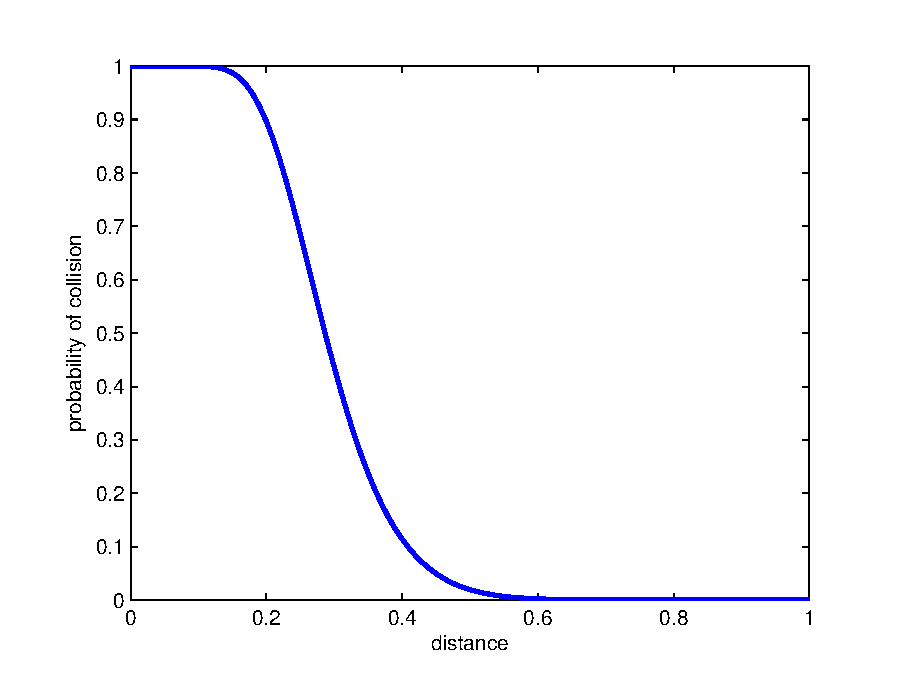
\includegraphics[width=0.5\textwidth]{pic_lsh_curve.eps}
    \caption{Пример зависимости вероятности того, что два объекта будут признаны алгоритмом как схожие,
        от расстояния между этими объектами.}
    \label{pic:lshCurve}
\end{figure}

Итоговый алгоритм является~$(d_1, d_2, 1 - (1 - p_1^m)^L, 1 - (1 - p_2^m)^L)$-чувствительным.
Вид зависимости вероятности коллизии от расстояния между объектами приведен
на рис.~\ref{pic:lshCurve}~(для~$m = 10$, $L = 20$).
Видно, что описанный способ композиции базовых хэш-функций позволяет добиться того,
что вероятность коллизии двух объектов как функция от расстояния имеет резкий скачок
в определенной точке~(в нашем примере~$0.7$).
За счет выбора параметров~$L$ и~$m$ можно менять положение точки скачка,
а также регулировать сложность алгоритма.
На практике эти параметры выбирают с помощью кросс-валидации.

Отметим также, что биты хэшей~$g_1(u), \dots, g_L(u)$ можно использоваться как признаки,
над которыми будет запускаться метод~$k$ ближайших соседей.

\paragraph{Теоретические гарантии.}
Будем говорить, что алгоритм решает задачу поиска~$c$-ближайшего соседа,
если для нового объекта~$u$ он с вероятностью~$1 - \eps$ возвращает объект выборки,
удаленный от~$u$ не более чем в~$c$ раз сильнее, чем ближайший к~$u$ объект выборки.
Существует теоретический результат, который говорит, что можно выбрать параметры~$L$ и~$m$
так, что описанный алгоритм будет решать задачу поиска~$c$-ближайшего соседа
за~$O(d \ell^r \log \ell)$, где~$r$ для многих функций расстояния имеет порядок~$1/c$~\cite{andoni08survey}.

\paragraph{Хэш-функции для косинусного расстояния.}
Для косинусного расстояния используют следующее семейство функций:
\[
    \FF
    =
    \{
        f_w(x) = \sign \langle w, x \rangle \cond w \in \RR^d
    \}.
\]
Каждая хэш-функция соответствует некоторой гиперплоскости, проходящей через
начало координат, и возвращает для каждого вектора либо~$+1$, либо~$-1$
в зависимости от того, по какую сторону от этой гиперплоскости он находится.

\paragraph{Хэш-функции для евклидовой метрики.}
В данном случае хэш-функция соответствует некоторой прямой в~$d$-мерном пространстве,
разбитой на отрезки длины~$r$.
Функция проецирует объект~$x$ на эту прямую и возвращает номер отрезка, в который попала проекция.
Формально, семейство хэш-функций имеет вид
\[
    \FF
    =
    \left\{
        f_{w, b}(x) = \left\lfloor \frac{\langle w, x \rangle + b}{r} \right\rfloor \cond w \in \RR^d, b \in [0, r)
    \right\}.
\]
При этом, в отличие от описанных выше семейств, функции выбираются не равномерно:
каждая компонента проекционного вектора~$w$ выбирается из стандартного нормального
распределения~$\mathcal{N}(0, 1)$.

Данное семейство может быть обобщено на расстояния Минковского с~$p \in (0, 2]$.
В этом случае компоненты вектора~$w$ должны выбираться из~$p$-устойчивого распределения~\cite{datar04pstable}.
Например, для~$p = 1$ таковым является распределение Коши.

\paragraph{LSH forest.}
В методе LSH присутствует два параметра: размерность хэша~$m$ и число хэшей~$L$.
Оба следует подбирать под конкретную задачу, и от их выбора может сильно
зависеть качество поиска соседей.
Один из вариантов решения~--- алгоритм~\emph{LSH forest}~\cite{bawa05lshforest},
в котором предлагается применить каждую хэш-функцию~$g_i$ к выборке
и построить префиксное дерево на её выходах.
Затем в качестве ближайших соседей для нового объекта объявляются те объекты из выборки,
с которыми он оказался в наиболее глубоких листовых вершинах.
Такой подход позволяет устранить зависимость от размера хэша и количества хэш-функций
и получать хорошее качество при их фиксированных значениях.

\paragraph{Рандомизированные алгоритмы.}
Подходы вроде locality-sensitive hashing достаточно популярны и используются для решения многих задач.
Так, \emph{фильтр Блума} позволяет с помощью небольшого числа бит и семейства хэш-функций
описать множество и проверять любой элемент на принадлежность ему.
Алгоритм~\emph{HyperLogLog} может приближенно найти число различных элементов в последовательности,
используя хэш-функции.
Во всех этих методах используется одна и та же идея: охарактеризовать сложную структуру с помощью некоторого количества
случайных признаков, и затем использовать только их для поиска нужной величины.

\paragraph{Обучение хэшированию.}
Рандомизированные методы простые в реализации и применении, но обладают существенным недостатком~---
никак не зависят от данных и от задачи, для решения которой используются.
Легко представить ситуацию, в которой все объекты сосредоточены в небольшом густом облаке,
и максимальный угол между двумя объектами составляет 10 градусов.
В этом случае большинство хэширующих гиперплоскостей, генерируемых для косинусного расстояния,
будут бесполезны.
Было бы разумно выбирать их так, чтобы они попадали в облако объектов.

На решение этой проблемы направлены методы~\emph{обучения хэшированию}~\cite{wang15survey}.
Их изложение выходит за рамки этого текста~--- отметим лишь, что они зачастую позволяют
существенно уменьшить число бит в хэше при сохранении точности поиска ближайших соседей.

\begin{thebibliography}{1}
\bibitem{weber98similarity}
    \emph{Weber, R., Schek, H. J.,  Blott, S.} (1998).
    A Quantitative Analysis and Performance Study for Similarity-Search Methods
    in High-Dimensional Spaces.~// Proceedings of the 24th VLDB Conference, New York C, 194–205.

\bibitem{andoni08survey}
    \emph{Andoni, A., Indyk, P.} (2008).
    Near-optimal hashing algorithms for approximate nearest neighbor in high dimensions.~//
    Communications of the ACM, 51(1), 117.
    
\bibitem{datar04pstable}
    \emph{Datar, M., Immorlica, N., Indyk, P., Mirrokni, V. S.} (2004).
    Locality-sensitive hashing scheme based on p-stable distributions.~//
    Proceedings of the twentieth annual symposium on Computational geometry - SCG  ’04, 253.

\bibitem{bawa05lshforest}
    \emph{Bawa, Mayank and Condie, Tyson and Ganesan, Prasanna} (2005).
    LSH Forest: Self-tuning Indexes for Similarity Search.~//
    Proceedings of the 14th International Conference on World Wide Web.
    
\bibitem{wang15survey}
    \emph{Wang, J., Liu, W., Kumar, S., Chang, S.-F.} (2015).
    Learning to Hash for Indexing Big Data - A Survey. \url{http://arxiv.org/abs/1509.05472}

\end{thebibliography}

\end{document}
